\section{Communiquer avec la base de données}

\subsection{DAO}

\subsubsection{Présentation}
Un objet d'accès aux données (Data Access Object ou DAO en anglais) est un modèle qui permet d'isoler les méthodes concernant le stockage des données et de ne pas les écrire directement dans nos classes métier. Ainsi le modèle DAO permet de regrouper l'accès aux données dans des classes à part plutôt que de les disperser. \\

Le but du modèle DAO est d'arriver à encapsuler les méthodes concernant la communication avec la base de données dans une coucher pour arriver au schéma suivant :

\begin{center}
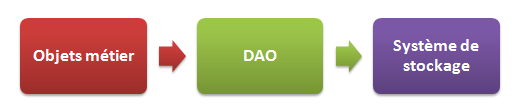
\includegraphics[scale=0.5]{../graph/dao1.png} \\
\end{center}

\subsubsection{Mise en place}
La couche DAO va gérer les opérations classiques de stockage : ajout, lecture, modification et suppression. Ces quatre opérations sont souvent raccourcis par l'acronyme CRUD (create, read, update and delete). \\

Pour mettre en application le modèle DAO nous avons du créer nos propres exceptions. En effet, il faut que les exceptions générées par SQL ou JDBC soit référencées comme étant des exceptions dues à la boite noire DAO. 

En reprenant la même idée, DAO se propose d'offrir une interface pour chacun des objets décrivant l'ensemble des méthodes qui seront accessibles dans l'objet. Ainsi, peu importe l'implémentation effectuée on pourra connaître les diverses méthodes de nos classes. Les interfaces permettent de décrire les méthodes des objets la couche donnée et ce n'est que l'implémentation qui sera dépendante du mode de stockage. \\ 
\begin{center}
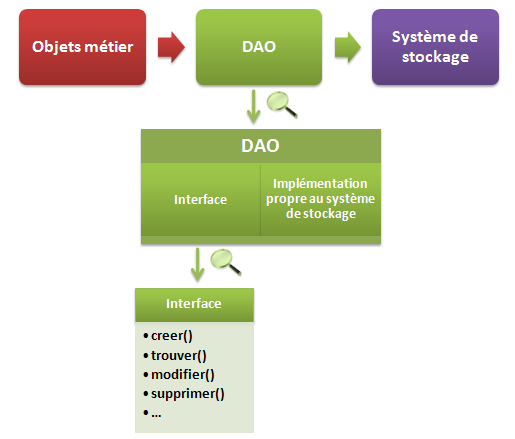
\includegraphics[scale=0.5]{../graph/dao2.png} \\
\end{center}

La couche DAO comportera également une fabrique. Cette fabrique sera unique et ne sera instanciée que si les informations de configuration sont correctes. Le but de cette fabrique sera de fournir une instance des différentes implémentations de la DAO.

\subsubsection{Avantage et Inconvénient}
L'avantage du modèle DAO est donc clair, le changement du stockage du mode de stockage de données est simple. En effet, nous aurons seulement à changer nos classes DAO pour changer ce mode de stockage. L'inconvénient est du à la mise en œuvre qui demande une couche supplémentaire. 


\subsection{La sérialisation}

\subsection{Principe}

La sérialisation est le processus de conversion d'un objet pour l'enregistrer dans une base de données ou un fichier par exemple. Le processus inverse s'appelle la désérialisation. Nous pouvons donc représenter cette méthode selon le schéma suivant. 

\begin{center}
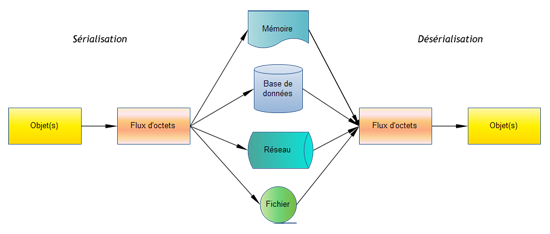
\includegraphics[scale=0.5]{../graph/serialisation.png} \\
\end{center}

\subsection{Mise en place}
On peut choisir par exemple d'effectuer sa sérialisation en XML. \\

La classe XMLEncoder permet de sérialiser un objet en XML. Cette sérialisation ne prend en compte que les champs ayant un getter et un setter public. XMLEncoder(output) crée une nouvelle instance qui utilise le flux passé en paramètre comme résultat de la sérialisation. \\

La classe XMLDecoder permet quand à elle de désérialiser un objet à partir d'un document XML. \\

Pour notre application nous aurions besoin d'effectuer une sérialisation vers SQL. Prenons l'exemple du joueur, pour effectuer la sérialisation nous avons besoin d'une classe Joueur qui implémente Serializable, d'avoir un constructeur par défaut et d'avoir un getter et un setter public pour chaque attribut. Ensuite notre table SQL java devrait contenir un id et un longblob (Binary Large Object). Ensuite nous n'aurions plus qu'a effectue une sauvegarde dans la base de données. Pour la desérialisation 


\subsection{Avantage et Inconvénient}
La sérialisation en XML présente des avantages comme une bonne portabilité ou le fait que le processus de sérialisation ne prenne pas en compte les champs qui ont leur valeur par défaut. Elle présente les inconvénients suivants : 
\begin{itemize}
\item ne peut s'utiliser que sur des objets respectant la convention JavaBeans (constructeur par défaut, getter et setter pour tous les attributs ..)
\item la taille des données sérialisés est plus importante que leur équivalent binaire
\end{itemize}